%%%%%%%%%%%%%%%%%%%%%%%%%%%%%%%%%%%%%%%%%%%%%%%%%%%%%
%%% Task 1 %%%%%%%%%%%%%%%%%%%%%%%%%%%%%%%%%%%%%%%%%%
%%%%%%%%%%%%%%%%%%%%%%%%%%%%%%%%%%%%%%%%%%%%%%%%%%%%%
\task{Fundamentals}

%%%%%%%%%%%%%%%%%%%%%%%%%%%%%%%%%%%%%%%%%%%%%%
\taskGerman{Grundlagen}

\begin{figure}[h!]
    \centering
    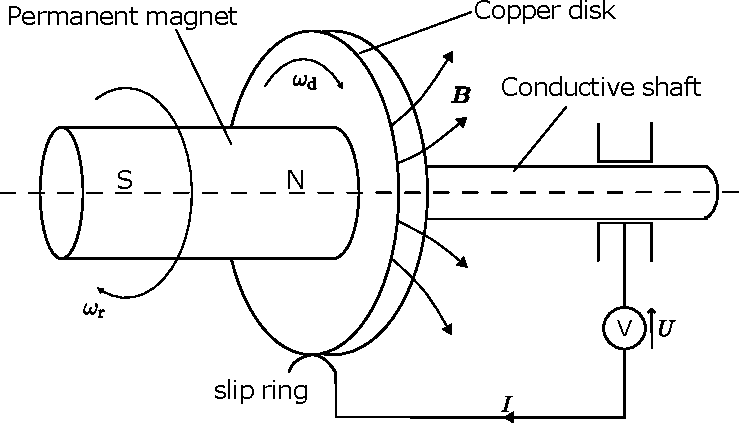
\includegraphics[width=0.6\textwidth]{fig/Faradays_disc.pdf}
    \caption{Faraday's disk (rotating copper disk in a homogenous magnetic field)}
    \label{fig:faraday_disk}
\end{figure}



\subtask{The disc from \autoref{fig:faraday_disk} has a diameter of $d=\SI{60}{\cm}$ and is rotating with the circumferential speed $v_\mathrm{d} = \SI{100}{\meter\per\second}$. What is the rotational speed and angular velocity of the copper disk?}{2}
\subtaskGerman{Die Scheibe aus \autoref{fig:faraday_disk} hat einen Durchmesser von $d=\SI{60}{\cm}$ und ihre Oberfläche rotiert mit der Umfangsgeschwindigkeit $v_\mathrm{d} = \SI{100}{\meter\per\second}$. Wie groß ist die Drehzahl $n_\mathrm{d}$ und die Winkelgeschwindigkeit $\omega_\mathrm{d}$ der Kupferscheibe?}

\begin{solutionblock}
    The rotational speed is given by
    $$ n_\mathrm{d} = \frac{v_\mathrm{d}}{2\pi r} = \frac{\SI{100}{\meter\per\second}\cdot \SI{60}{\second\per\minute}}{2\pi \cdot \SI{0.3}{\meter}} = \SI{3183}{\per\minute}.$$
    The angular velocity is
    $$ \omega_\mathrm{d} = 2\pi n_\mathrm{d} \SI{\frac{1}{60}}{\minute\per\second} = \SI{333}{\per\second}.$$
\end{solutionblock}


\subtask{Assuming that the permanent magnet is not rotating ($\omega_\mathrm{r}=0$) while delivering a homogenous and constant magnetic field with $B=\SI{1.8}{\tesla}$, what is the measured induced voltage $U$?}{2}
\subtaskGerman{Angenommen, dass der Permanentmagnet nicht rotiert ($\omega_\mathrm{r}=0$) allerdings ein homogenes und konstantes Magnetfeld mit $B=\SI{1.8}{\tesla}$ liefert, wie groß ist die gemessene induzierte Spannung $U$?}

\begin{solutionblock}
    Faraday's law of induction reads 
    $$u_\mathrm{i} =\oint_{\partial\mathcal{S}} \bm{E} \cdot \mathrm{d}\bm{s}$$ 
    where $\bm{E}$ is the electric field and $\partial\mathcal{S}$ is the boundary of the surface $\mathcal{S}$, which is the copper disk in this case. The electric field is a result of the rotating copper disk within the static magnetic field pointing from the center to the edge of the disk along the radial direction:
    $$\bm{E} = \bm{v} \times \bm{B} = v(r) B \bm{e}_\mathrm{r} .$$
    Here, $\bm{v}(r) = 2 \pi r n_\mathrm{d}$ is the velocity field of the disk for a given radius element $r$ and $\bm{e}_\mathrm{r}$ is the unit vector in the radial direction. The induced voltage is then
    \begin{align*}
        u_\mathrm{i} &= \int_{0}^{d/2} v(r) B \mathrm{d}r = B \int_{r=0}^{d/2} 2 \pi r n_\mathrm{d} \mathrm{d}r = 2 \pi Bn_\mathrm{d} \left[\frac{r^2}{2}\right]_{0}^{d/2} = \pi B n_\mathrm{d} \frac{d^2}{4} = \pi \cdot \SI{1.8}{\tesla} \cdot \SI{53.05}{\per\second}\cdot \SI{0.09}{\meter} \\&= \SI{27}{\volt}.
    \end{align*}
\end{solutionblock}

\subtask{Assume that the volt meter is exchanged for a resistor with $R=\SI{1}{\ohm}$. How big are the resulting current $I$ and electrical power $P$? Is the disc operating as a motor or generator?}{2}
\subtaskGerman{Nehmen Sie nun an, dass das Spannungsmessgerät durch einen Widerstand mit $R=\SI{1}{\ohm}$ ersetzt wird. Wie groß sind der resultierende Strom $I$ und die elektrische Leistung $P$? Funktioniert die Scheibe als Motor oder Generator?}

\begin{solutionblock}
    The current is given by Ohm's law $$I = -U/R = \SI{-27}{\volt}/\SI{1}{\ohm} = \SI{-27}{\ampere}.$$ The current is to be counted negative as the voltage and current in the above figure are oriented in opposite directions (load convention). The electrical power is $$P = I U = \SI{27}{\ampere} \cdot \SI{-27}{\volt} = \SI{-729}{\watt}.$$ The disc is operating as a generator, since the mechanical energy (which is introduced to rotate the disc) is converted into electrical energy. Also, there is no electrical energy source to power the disc, so it cannot operate as a motor.
\end{solutionblock}



\subtask{Discuss the three following cases regarding the presence of an induced voltage:}{2}
\begin{itemize}    
    \item The disc is at standstill, but the permanent magnet is rotating.
    \item The disc and the permanent magnet are rotating, but with different speeds.
    \item The disc and the permanent magnets are at standstill, but the  electrical circuit is rotating. 
\end{itemize}
\subtaskGerman{Diskutieren Sie die drei folgenden Fälle bezüglich der Präsenz einer induzierten Spannung $U$: \begin{itemize}
    \item Die Scheibe steht still, aber der Permanentmagnet rotiert.
    \item Die Scheibe und der Permanentmagnet rotieren, aber mit unterschiedlichen Geschwindigkeiten.
    \item Die Scheibe und die Permanentmagneten stehen still, aber der  elektrische Stromkreis rotiert.
\end{itemize}}

\begin{solutionblock}
    \begin{itemize}
        \item In the first case, there is no induced voltage as the magnetic field of the magnet is symmetric around the rotation axis, that is, the flux through the disc remains constant despite the magnet's rotation.
        \item In the second case it is only important to note that the disc is rotating (like in the original setup), which is the important factor for the induced voltage. The relative speed between the disc and the magnetic is not relevant due to the discussed rotational symmetry of the magnetic field.
        \item In the third case, the electrical circuit rotates through the constant magnetic field of the magnets which is analogously to the original setup of a rotating disc. Consequently, in this final case also a voltage is induced.
    \end{itemize}
\end{solutionblock}